% =====================================================================
%  CSCI 3130 -- Formal Languages & Automata Theory
%  Mock Midterm Exam (with full solutions)
%  Covers: Ch 1-6 (Lectures 1-6): sets/proofs, languages & grammars,
%  DFA/NFA, regular expressions, regular grammars, closure properties,
%  pumping lemma, context-free grammars, parsing & ambiguity,
%  grammar transformations, Chomsky/Greibach normal forms, CYK.
%  Source material: github.com/gingersea/3130 (lec1..lec6.pdf)
% =====================================================================
\documentclass[11pt,a4paper]{article}
\usepackage[margin=2.3cm]{geometry}
\usepackage{amsmath,amssymb}
\usepackage{enumitem}
\usepackage[T1]{fontenc}
\usepackage{lmodern}
\usepackage{microtype}
\usepackage[svgnames]{xcolor}
\usepackage[breakable,skins]{tcolorbox}
\usepackage{fancyhdr}
\usepackage{tikz}
\usetikzlibrary{arrows.meta,automata,positioning}

\setlist{nosep,topsep=2pt}
\setlength{\parindent}{0pt}

\pagestyle{fancy}
\fancyhf{}
\fancyhead[L]{\small\color{SteelBlue}\textbf{CSCI 3130 -- Mock Midterm Examination}}
\fancyhead[R]{\small\textbf{Page \thepage}}
\fancyfoot[C]{\small Formal Languages \& Automata Theory \textbullet\ based on lectures by Tsung-Yi Ho (CUHK)}

% ---------- helpers ---------------------------------------------------
\newcommand{\E}{\varepsilon}
\newcommand{\SX}{\Sigma}

% question box ---------------------------------------------------------
\newcounter{prob}
\newenvironment{problem}[1][]{%
  \refstepcounter{prob}%
  \begin{tcolorbox}[enhanced,breakable,colback=white,colframe=SteelBlue!70!black,
      boxrule=0.8pt,arc=1.5mm,left=5pt,right=5pt,top=3pt,bottom=3pt,
      before skip=8pt,after skip=8pt,
      title={\textbf{Question \theprob\ (#1)}},fonttitle=\bfseries, coltitle=white,
      colbacktitle=SteelBlue!70!black, boxed title style={arc=1mm}]}
{\end{tcolorbox}}

% solution box ---------------------------------------------------------
\newenvironment{solution}{%
  \begin{tcolorbox}[enhanced,breakable,colback=Honeydew!55,colframe=ForestGreen!60!black,
      boxrule=0.6pt,arc=1.5mm,left=5pt,right=5pt,top=3pt,bottom=3pt,
      before skip=6pt,after skip=10pt,
      title={\textbf{Solution \theprob}},fonttitle=\bfseries, coltitle=white,
      colbacktitle=ForestGreen!60!black, boxed title style={arc=1mm}]}
{\end{tcolorbox}}

\newcommand{\RE}[1]{\texttt{#1}}
\newcommand{\ok}{\ensuremath{\checkmark}}

\begin{document}

\begin{center}
  {\LARGE\bfseries CSCI 3130 -- Formal Languages and Automata Theory}\\[2mm]
  {\large\bfseries Mock Midterm Examination}\\[1mm]
  {\normalsize Covering Lectures 1--6 (Chapters 1--6)} \\[2mm]
  {\small \textbf{Instructions:} Answer all questions in the space provided.
  Total: 100 points. Time suggested: 120 minutes. Closed book, no calculators.
  Unless stated otherwise, $\Sigma=\{a,b\}$ means the alphabet is $\{a,b\}$ and
  $\lambda$ denotes the empty string.}\\[4mm]
  \begin{tabular}{@{}ll@{}}
    \textbf{Question} & \textbf{Points}\\
    Q1. Mathematical Preliminaries \& Proofs & 10 \\
    Q2. Languages and Grammars & 12 \\
    Q3. Deterministic Finite Accepters (DFA) & 14 \\
    Q4. Nondeterministic Finite Accepters (NFA) & 14 \\
    Q5. Regular Expressions \& Regular Grammars & 12 \\
    Q6. Closure Properties \& Decision Questions & 12 \\
    Q7. Pumping Lemma & 14 \\
    Q8. Context-Free Grammars \& Normal Forms & 12 \\
    \hline
    \textbf{Total} & \textbf{100}\\
  \end{tabular}
\end{center}

\vspace{2mm}
\noindent\rule{\linewidth}{0.6pt}
\vspace{1mm}
{\color{SteelBlue}\bfseries\large Part I -- Questions}\\[2mm]
\noindent\rule{\linewidth}{0.6pt}

%======================================================================
\begin{problem}[Mathematical Preliminaries and Proofs -- 10 points]
\begin{enumerate}[label=(\alph*)]
  \item (2 pts) Let $A=\{1,2,3\}$ and $B=\{2,3,4,5\}$. Compute
  $A\cup B$, $A\cap B$, $A-B$, and the powerset $2^B$ restricted to
  subsets of size 2. How many subsets does $2^B$ have in total?
  \item (2 pts) Use DeMorgan's laws to simplify
  $\overline{(A\cap B)\cup C}$ into a form with no complement applied
  to a union or intersection, given a universe $U$. (Write the answer
  using complements of single sets only.)
  \item (3 pts) Prove by induction that a binary tree of height $n$
  has at most $2^n$ leaves. State the basis, the inductive hypothesis,
  and the inductive step explicitly.
  \item (3 pts) Prove by contradiction that $\sqrt{2}$ is not rational.
\end{enumerate}
\end{problem}

\begin{solution}
\begin{enumerate}[label=(\alph*)]
  \item $A\cup B=\{1,2,3,4,5\}$; $A\cap B=\{2,3\}$; $A-B=\{1\}$
  (and $B-A=\{4,5\}$). The subsets of $B$ of size 2 are
  $\{2,3\},\{2,4\},\{2,5\},\{3,4\},\{3,5\},\{4,5\}$. Since
  $|B|=4$, the powerset has $|2^B|=2^{|B|}=2^4=16$ subsets.
  \item By DeMorgan:
  $\overline{(A\cap B)\cup C}=\overline{A\cap B}\cap\bar C
  =(\bar A\cup\bar B)\cap\bar C$.
  \item \textbf{Theorem:} a binary tree of height $n$ has at most
  $2^n$ leaves. Let $L(i)$ = maximum number of leaves of a subtree at
  height $i$. \textbf{Basis:} $L(0)=1$ (the root alone).
  \textbf{Hypothesis:} assume $L(i)\le 2^i$ for all $i=0,1,\dots,k$.
  \textbf{Step:} a subtree of height $k+1$ consists of a root with at
  most two children, each the root of a subtree of height at most $k$,
  so $L(k+1)\le 2\cdot L(k)\le 2\cdot 2^k=2^{k+1}$. Done.
  \item Assume $\sqrt2$ is rational: $\sqrt2=n/m$ with $n,m$
  integers having no common factors. Then $2m^2=n^2$, so $n^2$ is
  even, hence $n$ is even, $n=2k$. Then $2m^2=4k^2$, i.e.\ $m^2=2k^2$,
  so $m^2$ is even and hence $m$ is even, $m=2p$. Thus $n$ and $m$
  share the factor 2, contradicting that they have no common factors.
  Therefore $\sqrt2$ is not rational. \hfill$\blacksquare$\ 
\end{enumerate}
\end{solution}

%======================================================================
\begin{problem}[Languages and Grammars -- 12 points]
Let $\Sigma=\{a,b\}$ and let $L=\{a^nb^n:n\ge0\}$.
\begin{enumerate}[label=(\alph*)]
  \item (2 pts) Is $\lambda\in L$? Is $aab\in L$? Is $aabbaaabbb\in L^2$? Justify briefly.
  \item (3 pts) Give a grammar $G$ with $L(G)=L$ and show a derivation of $aabb$ in $G$. Identify one sentential form and one sentence in your derivation.
  \item (3 pts) Give a grammar for $L'=\{a^nb^{n+1}:n\ge0\}$ and briefly explain why it works.
  \item (2 pts) Consider $G'':\ S\to SS\ |\ \lambda\ |\ aSb\ |\ bSa$ over $\{a,b\}$.
  What language does $G''$ generate? (You do not need a full proof, but name the language.)
  \item (2 pts) When are two grammars $G_1$ and $G_2$ said to be \emph{equivalent}? Give an example of two different (non-identical production sets) equivalent grammars.
\end{enumerate}
\end{problem}

\begin{solution}
\begin{enumerate}[label=(\alph*)]
  \item $\lambda=a^0b^0$, so $\lambda\in L$. $aab\notin L$ (the
  numbers of $a$'s and $b$'s differ). $L^2=\{a^nb^na^mb^m:n,m\ge0\}$,
  and with $n=2$, $m=3$: $aabbaaabbb=a^2b^2a^3b^3\in L^2$. Yes.
  \item $G=(\{S\},\{a,b\},S,P)$ with $P=\{S\to aSb,\ S\to\lambda\}$.
  Derivation: $S\Rightarrow aSb\Rightarrow aaSbb\Rightarrow aabb$.
  Sentential forms: $S$, $aSb$, $aaSbb$ (e.g.\ $aaSbb$ contains the
  variable $S$). Sentence: $aabb$ (all terminals).
  \item $G'=(\{S,A\},\{a,b\},S,P')$ with $S\to Ab$, $A\to aAb$,
  $A\to\lambda$. Applying $A\to aAb$ $n$ times and then $A\to\lambda$
  gives $a^nb^n$, and the final $S\to Ab$ appends one extra $b$:
  $L(G')=\{a^nb^{n+1}:n\ge0\}$. Example: $S\Rightarrow Ab\Rightarrow aAbb\Rightarrow aabb$.
  \item $L(G'')=\{w\in\{a,b\}^*:n_a(w)=n_b(w)\}$ -- all strings with
  the same number of $a$'s and $b$'s (proof by induction on $|w|$:
  if $w$ starts and ends with different letters, peel them with
  $aSb$/$bSa$; otherwise split $w=w_1w_2$ and use $S\to SS$).
  \item $G_1$ and $G_2$ are equivalent iff $L(G_1)=L(G_2)$. Example:
  $G_1:\ S\to aSb\ |\ \lambda$ and $G_2:\ S\to aAb\ |\ \lambda,\ A\to aAb\ |\ \lambda$;
  both generate $\{a^nb^n:n\ge0\}$.
\end{enumerate}
\end{solution}

%======================================================================
\begin{problem}[Deterministic Finite Accepters -- 14 points]
\begin{enumerate}[label=(\alph*)]
  \item (4 pts) Design a DFA over $\Sigma=\{0,1\}$ that accepts
  exactly the strings that contain the substring $001$. Draw the state
  diagram.
  \item (4 pts) Write the 5-tuple $M=(Q,\Sigma,\delta,q_0,F)$ for
  your DFA in (a) using a transition table.
  \item (3 pts) For a DFA, define the extended transition function
  $\delta^*$ and the language $L(M)$. Illustrate with $\delta^*(q_0,00110)$
  in your machine.
  \item (3 pts) Design a DFA for
  $L=\{w\in\{a,b\}^*:\ |w|\bmod 3=0\}$. How many states do you need? Why is this number minimal?
\end{enumerate}
\end{problem}

\begin{solution}
\begin{enumerate}[label=(\alph*)]
  \item States remember the longest prefix of $001$ seen so far:
  $q_0$ (no progress), $q_1$ (seen $0$), $q_2$ (seen $00$),
  $q_3$ (seen $001$, accepting trap, loops on $0,1$).
  Transitions: $q_0\overset{0}{\to}q_1$, $q_0\overset{1}{\to}q_0$;
  $q_1\overset{0}{\to}q_2$, $q_1\overset{1}{\to}q_0$;
  $q_2\overset{0}{\to}q_2$, $q_2\overset{1}{\to}q_3$;
  $q_3\overset{0,1}{\to}q_3$.

  \begin{center}
  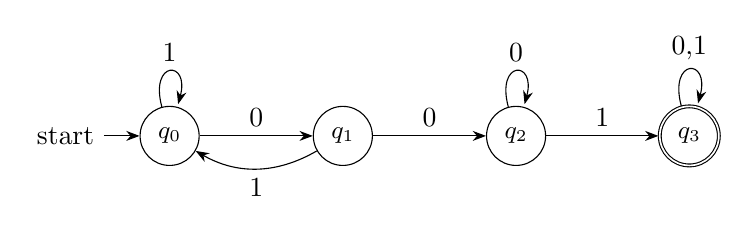
\begin{tikzpicture}[>=Stealth, node distance=2.2cm, on grid, auto,
      every state/.style={draw,circle,minimum size=7.5mm,inner sep=1pt,font=\small}]
    \node[state,initial] (q0) {$q_0$};
    \node[state] (q1) [right=of q0] {$q_1$};
    \node[state] (q2) [right=of q1] {$q_2$};
    \node[state,accepting] (q3) [right=of q2] {$q_3$};
    \path[->] (q0) edge [loop above] node {1} (q0)
              (q0) edge node {0} (q1)
              (q1) edge [bend left] node {1} (q0)
              (q1) edge node {0} (q2)
              (q2) edge [loop above] node {0} (q2)
              (q2) edge node {1} (q3)
              (q3) edge [loop above] node {0,1} (q3);
  \end{tikzpicture}
  \end{center}

  \item $M=(Q,\Sigma,\delta,q_0,F)$ with $Q=\{q_0,q_1,q_2,q_3\}$,
  $\Sigma=\{0,1\}$, $F=\{q_3\}$:

  \begin{center}
  \begin{tabular}{c|cc}
  $\delta$ & 0 & 1\\ \hline
  $q_0$ & $q_1$ & $q_0$\\
  $q_1$ & $q_2$ & $q_0$\\
  $q_2$ & $q_2$ & $q_3$\\
  $q_3$ & $q_3$ & $q_3$\\
  \end{tabular}
  \end{center}

  \item Recursive definition: $\delta^*(q,\lambda)=q$ and
  $\delta^*(q,wa)=\delta(\delta^*(q,w),a)$. Language:
  $L(M)=\{w\in\Sigma^*:\delta^*(q_0,w)\in F\}$. For $w=00110$:
  $\delta^*(q_0,0)=q_1$, $\delta^*(q_0,00)=q_2$,
  $\delta^*(q_0,001)=q_3$, and from $q_3$ the machine loops, so
  $\delta^*(q_0,00110)=q_3\in F$: $00110$ is accepted (it contains
  the substring $001$).
  \item Use a 3-state cycle counting $|w|\bmod 3$: states $0,1,2$,
  start 0, final $\{0\}$, $\delta(i,a)=\delta(i,b)=(i+1)\bmod 3$.
  Three states are minimal: the states reached by $\lambda$, $a$,
  $aa$ must be pairwise distinguishable. Reached by $\lambda$ vs
  $a$: reading $\lambda$, the first ends final, the second does not.
  Reached by $a$ vs $aa$: reading $b$, we reach state
  $|ab|=2$ (non-final) vs state $|aab|=3$ (final). Three pairwise
  distinguishable states force at least 3 states.
\end{enumerate}
\end{solution}

%======================================================================
\begin{problem}[Nondeterministic Finite Accepters -- 14 points]
Consider the NFA $M$ with $\Sigma=\{a,b\}$:

\begin{center}
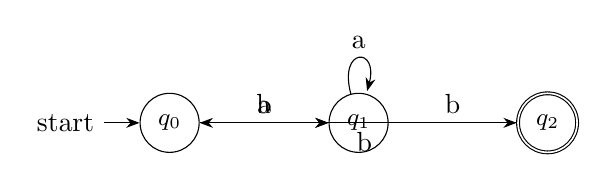
\begin{tikzpicture}[>=Stealth, node distance=2.4cm, on grid, auto,
    every state/.style={draw,circle,minimum size=7.5mm,inner sep=1pt,font=\small}]
  \node[state,initial] (q0) {$q_0$};
  \node[state] (q1) [right=of q0] {$q_1$};
  \node[state,accepting] (q2) [right=of q1] {$q_2$};
  \path[->] (q0) edge node {a} (q1)
            (q0) edge node {b} (q1)
            (q1) edge [loop above] node {a} (q1)
            (q1) edge node {b} (q2)
            (q2) edge node {\;\,b} (q0);
\end{tikzpicture}
\end{center}

\begin{enumerate}[label=(\alph*)]
  \item (3 pts) Give $\delta^*(q_0,a)$, $\delta^*(q_0,ab)$, and $\delta^*(q_0,aaabbb)$. Which of the strings $ab$, $aaabbb$, $abab$ are accepted?
  \item (3 pts) What is $L(M)$? Describe it in words and as a set or regular expression.
  \item (8 pts) Apply the subset construction to convert $M$ into an equivalent DFA $M'$. Show all DFA states, the transition function, the initial state, and the final states. Verify that $ab$ is accepted by $M'$.
\end{enumerate}
\end{problem}

\begin{solution}
\begin{enumerate}[label=(\alph*)]
  \item $\delta^*(q_0,a)=\{q_1\}$;
  $\delta^*(q_0,ab)=\{q_2\}$;
  for $aaabbb$: $q_0\overset{a}{\to}q_1\overset{a}{\to}q_1\overset{a}{\to}q_1\overset{b}{\to}q_2\overset{b}{\to}q_0\overset{b}{\to}q_1$,
  so $\delta^*(q_0,aaabbb)=\{q_1\}$.
  Accept: $ab\in L(M)$ since $\{q_2\}$ contains a final state;
  $aaabbb\notin L(M)$ (ends at $\{q_1\}$, not final);
  $abab$: after $ab$ we are at $q_2$, but $\delta(q_2,a)=\emptyset$
  -- the only computation hangs, so $abab\notin L(M)$.
  \item From the DFA computed in (c):
  $L(M)=\big((a\cup b)a^*bb\big)^*(a\cup b)a^*b$.
  In words: any number of ``round trips'': one letter, then any
  number of $a$'s, then exactly two $b$'s (the first $b$ reaches the
  final state, the second returns to the start state), followed by a
  final block: one letter, any number of $a$'s, and a single $b$
  ending in the final state.
  Check: $ab$: zero round trips plus final block $ab$ -- accepted. \ok
  \item Subset construction. NFA transitions: $\delta(q_0,a)=\delta(q_0,b)=\{q_1\}$; $\delta(q_1,a)=\{q_1\}$; $\delta(q_1,b)=\{q_2\}$; $\delta(q_2,b)=\{q_0\}$; all others $\emptyset$. DFA $M'$:
  Start $A=\{q_0\}$.
  $\delta'(A,a)=\{q_1\}=B$; $\delta'(A,b)=\{q_1\}=B$.
  $B=\{q_1\}$: $\delta'(B,a)=\{q_1\}=B$; $\delta'(B,b)=\{q_2\}=C$.
  $C=\{q_2\}$: $\delta'(C,a)=\emptyset=D$; $\delta'(C,b)=\{q_0\}=A$.
  $D=\emptyset$: loops on $a,b$.
  Final states of $M'$: states containing $q_2$, i.e.\ $F'=\{C\}$.
  $ab$: $A\overset{a}{\to}B\overset{b}{\to}C\in F'$: accepted. \ok
  (This DFA confirms the language in (b): loops $A\to B\overset{a^*}{\longrightarrow}B\overset{b}{\to}C\overset{b}{\to}A$
  plus the exit $A\to B\overset{a^*}{\longrightarrow}B\overset{b}{\to}C$.)
\end{enumerate}
\end{solution}

%======================================================================
\begin{problem}[Regular Expressions and Regular Grammars -- 12 points]
\begin{enumerate}[label=(\alph*)]
  \item (3 pts) Give a regular expression over $\Sigma=\{0,1\}$ for
  $L_1=\{w: w$ contains at least one pair of consecutive 0s$\}$.
  \item (3 pts) Give a regular expression for
  $L_2=\{w\in\{0,1\}^*: w$ does not end in $01\}$.
  \item (3 pts) Give a regular expression for
  $L_3=\{w\in\{a,b\}^*: n_a(w)$ is even$\}$.
  \item (3 pts) Consider the right-linear grammar
  $G:\ V_0\to aV_1,\ V_1\to abV_0\ |\ b$. Construct an NFA that accepts
  $L(G)$ and give $L(G)$ as a regular expression.
\end{enumerate}
\end{problem}

\begin{solution}
\begin{enumerate}[label=(\alph*)]
  \item $r_1=(0+1)^*00(0+1)^*$ (anything, then $00$, then anything).
  \item If $x$ does not end in $01$, then $|x|<2$ or $x$ ends in
  $00$, $10$, or $11$: $r_2=\lambda+0+1+(0+1)^*(00+10+11)$.
  \item Express $x$ as blocks around each odd occurrence pattern:
  an even number of $a$'s means: some $b$'s, then pairs of $a$'s
  separated by arbitrary $b$'s: $r_3=b^*(ab^*ab^*)^*$, equivalently
  $(b^*ab^*a)^*b^*$ or $(b+ab^*a)^*$.
  \item From $G$: variables $V_0,V_1$ become NFA states, plus final
  state $V_F$; start $V_0$. $V_0\to aV_1$: edge $V_0\overset{a}{\to}V_1$.
  $V_1\to abV_0$: chain $V_1\overset{a}{\to}X\overset{b}{\to}V_0$.
  $V_1\to b$: edge $V_1\overset{b}{\to}V_F$ ($V_F$ final).
  $L(G)=(aab)^*ab$ (the loop $a\,a\,b$ returns to $V_0$; the exit
  $a\,b$ leads to the final state).
\end{enumerate}
\end{solution}

%======================================================================
\begin{problem}[Closure Properties and Decision Questions -- 12 points]
\begin{enumerate}[label=(\alph*)]
  \item (3 pts) Let $L_1=\{a^nb:n\ge0\}$ and $L_2=\{ba\}$, both regular. Using only the standard NFA constructions (union, concatenation, star, reversal), build an NFA for $L_1^R\cup L_1L_2$. Sketch the construction (state diagrams) and state what language the result accepts.
  \item (4 pts) For DFAs $M_1=(Q_1,\Sigma,\delta_1,q_1,F_1)$ and
  $M_2=(Q_2,\Sigma,\delta_2,q_2,F_2)$, write down the product DFA $M$
  that accepts $L(M_1)-L(M_2)$, giving $Q$, $\delta$, $q_0$, and $F$.
  (Note: for the complement construction, a DFA must be complete --
  add a trap state if some transitions are missing.)
  \item (2 pts) Given a regular language $L$ (by its DFA), how do you decide each of the following: (i) $w\in L$; (ii) $L=\emptyset$; (iii) $L$ is infinite.
  \item (3 pts) Let $h:\{a,b\}\to\{a,b,c\}^*$ be the homomorphism with $h(a)=ab$, $h(b)=bbc$. Compute $h(aba)$ and the homomorphic image of the language denoted by $r=(a+b^*)(aa)^*$.
\end{enumerate}
\end{problem}

\begin{solution}
\begin{enumerate}[label=(\alph*)]
  \item $L_1=\{a^nb:n\ge0\}$ has NFA $M_1$: $q_0\overset{a}{\circlearrowleft}\overset{b}{\to}q_f$.
  $L_1^R=\{ba^n:n\ge0\}$: reverse all transitions and swap
  initial/final: $q_f$ becomes initial: $q_f\overset{b}{\to}q_0$,
  $q_0\overset{a}{\circlearrowleft}$, with $q_0$ final (and add a new
  single final state if needed). $L_1L_2=\{a^nbba:n\ge0\}$:
  concatenate $M_1$ with $M_2$ ($M_2$: $p_0\overset{b}{\to}p_1\overset{a}{\to}p_2$)
  via a $\lambda$-edge from $q_f$ to $p_0$, final state $p_2$. Then
  $L_1^R\cup L_1L_2$: new start with $\lambda$-edges into both
  machines and a single new final state. Result:
  $\{ba^n:n\ge0\}\cup\{a^nbba:n\ge0\}$.
  \item $M=(Q_1\times Q_2,\Sigma,\delta,(q_1,q_2),F)$ where
  $\delta((p,q),a)=(\delta_1(p,a),\delta_2(q,a))$ and
  $F=\{(p,q):p\in F_1\ \text{and}\ q\notin F_2\}$. (Equivalently
  $L_1\cap\bar L_2$.)
  \item (i) Simulate the DFA on $w$; accept iff the final state
  $\delta^*(q_0,w)\in F$. (ii) $L=\emptyset$ iff no final state is
  reachable from $q_0$ (graph reachability). (iii) $L$ is infinite
  iff some final state is reachable from $q_0$ via a walk containing
  a cycle; otherwise finite.
  \item $h(aba)=h(a)h(b)h(a)=ab\,bbc\,ab=abbbcab$.
  The language denoted by $r=(a+b^*)(aa)^*$ is
  $L(r)=\{a,b,b^2,b^3,\ldots\}\{a^{2n}:n\ge0\}$. By Theorem 4.3 the
  homomorphic image is regular and is denoted by substituting the
  images of the letters into $r$:
  $h(r)=\big(ab+(bbc)^*\big)(abab)^*$.
\end{enumerate}
\end{solution}

%======================================================================
\begin{problem}[Pumping Lemma -- 14 points]
\begin{enumerate}[label=(\alph*)]
  \item (2 pts) State the Pumping Lemma for regular languages, naming all three conditions on the decomposition $w=xyz$.
  \item (6 pts) Prove, using the Pumping Lemma, that
  $L=\{a^nb^n:n\ge0\}$ is not regular. Structure your proof as a game: what does the opponent give, what string do you pick, and what contradiction follows for \emph{every} possible decomposition?
  \item (6 pts) Prove that $L=\{a^p:p\text{ is prime}\}$ over $\Sigma=\{a\}$ is not regular.
\end{enumerate}
\end{problem}

\begin{solution}
\begin{enumerate}[label=(\alph*)]
  \item If $L$ is an infinite regular language, then there exists an
  integer $m$ such that every $w\in L$ with $|w|\ge m$ can be written
  $w=xyz$ with (1) $|xy|\le m$, (2) $|y|\ge1$, and (3)
  $xy^iz\in L$ for all $i=0,1,2,\ldots$
  \item Assume $L$ is regular. Let $m$ be the pumping constant.
  Pick $w=a^mb^m\in L$; $|w|=2m\ge m$. Consider any decomposition
  $w=xyz$ with $|xy|\le m$ and $|y|\ge1$. Since $|xy|\le m$, both
  $x$ and $y$ lie entirely in the $a$-part: $y=a^k$ for some
  $k\ge1$. Then $xy^2z=a^{m+k}b^m$. Since $k\ge1$, $m+k\neq m$, so
  $a^{m+k}b^m\notin L$, contradicting condition (3). Hence no such
  decomposition works and $L$ is not regular. \hfill$\blacksquare$\ 
  (Game form: $O$ gives $m$; $P$ picks $a^mb^m$; $O$ chooses
  $y=a^k$, $1\le k\le m$; $P$ pumps $i=2$ and wins.)
  \item Assume $L$ regular with constant $m$. Choose $p$ = the
  smallest prime $\ge m$, and pick $w=a^p\in L$. Any decomposition
  with $|xy|\le m$ gives $y=a^k$, $1\le k\le m$ (with $k\le p$).
  Pump $i=p+1$: $xy^{p+1}z=a^{p+pk}=a^{p(k+1)}$. Since $k\ge1$,
  $p(k+1)$ is composite, so $xy^{p+1}z\notin L$ -- contradiction.
  Hence $L$ is not regular. \hfill$\blacksquare$\ 
  (Equivalently, pump with $i-1=p$: length $p+(i-1)k=p(k+1)$.)
\end{enumerate}
\end{solution}

%======================================================================
\begin{problem}[Context-Free Grammars and Normal Forms -- 12 points]
\begin{enumerate}[label=(\alph*)]
  \item (2 pts) Give a CFG for $L=\{ww^R:w\in\{a,b\}^*\}$ and show a derivation of $abba$.
  \item (3 pts) Show that $E\to E+E\ |\ E*E\ |\ (E)\ |\ a$ is ambiguous by exhibiting two different leftmost derivations of $a+a*a$. Then write an equivalent unambiguous grammar.
  \item (3 pts) Convert $G:\ S\to ABa,\ A\to aab,\ B\to Ac$ into Chomsky normal form, showing the intermediate steps (terminal replacement and binarization).
  \item (4 pts) Apply the CYK algorithm to determine whether $w=aabbb$ is in $L(G)$ for the CNF grammar $S\to AB,\ A\to BB\ |\ a,\ B\to AB\ |\ b$. Show the dynamic programming table (the triangle of substring sets).
\end{enumerate}
\end{problem}

\begin{solution}
\begin{enumerate}[label=(\alph*)]
  \item $G:\ S\to aSa\ |\ bSb\ |\ \lambda$. Derivation:
  $S\Rightarrow aSa\Rightarrow abSba\Rightarrow abba$ (then
  $S\Rightarrow\lambda$). $abba=(ab)(ab)^R$? Indeed $abba$ with
  $w=ab$: $w^R=ba$, $ww^R=abba$. \ok
  \item Leftmost derivation 1:
  $E\Rightarrow E+E\Rightarrow a+E\Rightarrow a+E*E\Rightarrow a+a*E\Rightarrow a+a*a$.
  Leftmost derivation 2:
  $E\Rightarrow E*E\Rightarrow E+E*E\Rightarrow a+E*E\Rightarrow a+a*E\Rightarrow a+a*a$.
  Two distinct leftmost derivations $\Rightarrow$ ambiguous.
  Unambiguous grammar (precedence: $*$ binds tighter than $+$):
  $E\to E+T\ |\ T$; $T\to T*F\ |\ F$; $F\to (E)\ |\ a$.
  \item Step 1 (terminals): add $T_a\to a$, $T_b\to b$, $T_c\to c$;
  replace terminals in long productions:
  $S\to ABT_a$, $A\to T_aT_aT_b$, $B\to AT_c$, plus $T_a\to a,T_b\to b,T_c\to c$.
  Step 2 (binarize):
  $S\to ABT_a$ $\Rightarrow$ $S\to AV_1$, $V_1\to BT_a$.
  $A\to T_aT_aT_b$ $\Rightarrow$ $A\to T_aV_2$, $V_2\to T_aT_b$.
  $B\to AT_c$ is already in CNF.
  Final CNF grammar:
  $S\to AV_1$; $V_1\to BT_a$; $A\to T_aV_2$; $V_2\to T_aT_b$;
  $B\to AT_c$; $T_a\to a$; $T_b\to b$; $T_c\to c$.
  \item CNF: $S\to AB$, $A\to BB|a$, $B\to AB|b$; $w=aabbb$.
  Table $V_{ij}$ (variables deriving $w_i\cdots w_j$):
  \begin{center}
  \begin{tabular}{c|ccccc}
  length & \multicolumn{5}{c}{substrings}\\ \hline
  1 & $a\mapsto\{A\}$ & $a\mapsto\{A\}$ & $b\mapsto\{B\}$ & $b\mapsto\{B\}$ & $b\mapsto\{B\}$\\
  2 & $aa\mapsto\emptyset$ & $ab\mapsto\{S,B\}$ & $bb\mapsto\{A\}$ & $bb\mapsto\{A\}$ & \\
  3 & $aab\mapsto\{S,B\}$ & $abb\mapsto\{A\}$ & $bbb\mapsto\{S,B\}$ & & \\
  4 & $aabb\mapsto\{A\}$ & $abbb\mapsto\{S,B\}$ & & & \\
  5 & $aabbb\mapsto\{S,B\}$ & & & & \\
  \end{tabular}
  \end{center}
  Example: $ab\mapsto\{S,B\}$ since $S\to AB$ and $B\to AB$ with
  $A\in V_{11}$ and $B\in V_{22}$ ($a\mapsto A$, $b\mapsto B$).
  Since $S\in V_{15}$, $aabbb\in L(G)$. \ok
\end{enumerate}
\end{solution}

\vspace{3mm}
{\color{SteelBlue}\bfseries\large End of Examination}

\end{document}
